\documentclass[default]{beamer}
\setbeamertemplate{navigation symbols}{}

\usetheme{CambridgeUS}
\usecolortheme{beaver}

\usepackage[utf8]{inputenc}
\usepackage[english, russian]{babel}
\usepackage{csquotes}
\usepackage{animate}
\usepackage{fp}
\usepackage{textpos}
\usepackage{dtk-logos}

\usepackage{tikz}
\usetikzlibrary{arrows,shapes,calc}

\usepackage{xcolor}
\usepackage{listings}
\lstset
{
	language=[LaTeX]TeX,
	breaklines=true,
	basicstyle=\tt\scriptsize,
	keywordstyle=\color{blue},
	identifierstyle=\color{magenta},
}

\usepackage[
	language=auto,
	autolang=other,
	backend=biber,
	style=authortitle,
	sorting=ydnt,
	maxbibnames=5
]{biblatex}
\addbibresource{panov_latex.bib}

\DeclareSourcemap{
	\maps[datatype=bibtex, overwrite]{
		\map{
			\step[fieldset=langid, fieldvalue=english]
			\step[fieldset=doi, null]
			\step[fieldset=issn, null]
			\step[fieldset=isbn, null]
			\step[fieldset=url, null]
			\step[fieldsource=language, fieldset=langid, origfieldval]
		}
	}
}
\DeclareBibliographyDriver{std}{%
	\usebibmacro{bibindex}%
	\usebibmacro{begentry}%
	\usebibmacro{author/editor+others/translator+others}%
	\setunit{\labelnamepunct}\newblock
	\usebibmacro{title}%
	\newunit\newblock
	\usebibmacro{maintitle+booktitle}
	\newunit\newblock
	\usebibmacro{journal}%
	\newunit\newblock
	\usebibmacro{date}%
	\newunit\newblock
	\usebibmacro{finentry}
}
\DeclareBibliographyAlias{article}{std}
\DeclareBibliographyAlias{book}{std}
\DeclareBibliographyAlias{inproceedings}{std}
\DeclareBibliographyAlias{incollection}{std}

\graphicspath{{../../images/}} 			% Пути к изображениям

\makeatletter
\setbeamertemplate{footline}
{
	\leavevmode%
	\hbox{%
		\begin{beamercolorbox}[wd=.333333\paperwidth,ht=2.25ex,dp=1ex,center]{author
				in head/foot}%
			\usebeamerfont{author in
				head/foot}\insertshortauthor~~\beamer@ifempty{\insertshortinstitute}{}{(\insertshortinstitute)}
		\end{beamercolorbox}%
		\begin{beamercolorbox}[wd=.333333\paperwidth,ht=2.25ex,dp=1ex,center]{title in
				head/foot}%
			\usebeamerfont{title in head/foot}\insertshorttitle
		\end{beamercolorbox}%
		\begin{beamercolorbox}[wd=.333333\paperwidth,ht=2.25ex,dp=1ex,right]{date in
				head/foot}%
			\usebeamerfont{date in head/foot}\insertshortdate{}\hspace*{1em}
			\insertframenumber{}\hspace*{2ex} 
		\end{beamercolorbox}
	}%
	\vskip0pt%
}

\addtobeamertemplate{frametitle}{}{
	\begin{textblock*}{100mm}(\textwidth-35pt,-20pt)
		
\includegraphics[width=1.5cm]{misc/logos/frccsc.png}
	\end{textblock*}
}

\newcommand{\predmatr}[3]{
	\node[ell, rectangle, minimum height = 15, minimum width = 7.5]  at (#1 pt,#2 pt) {}; 
	\node[ellf, rectangle, minimum height = 15, minimum width = 7.5] at (#1+7.5 pt,#2 pt) {};
	\node[minimum height = 15, minimum width = 15] (#3) at (#1+3.3pt,#2 pt) {};
	\draw[ell] (#1+7.5 pt,#2+7.5 pt) -- (#1 +7.5 pt,#2-7.5 pt);
}
\renewcommand*{\bibfont}{\tiny}
\setlength\bibitemsep{-5pt}

\begin{document}
	
	\title[\LaTeX]{\LaTeX в научных публикациях и презентациях}
	\author[Панов]{Александр Панов}
	\institute[ФИЦ ИУ РАН]{Лаборатория интеллектуальных динамических систем\\Институт системного анализа\\ Федеральный исследовательский центр <<Информатика и управление>>\\Российской академии наук}
	\date{8 ноября -- Семинар СМУ} 
	
	\begin{frame}
		\titlepage
		\centering
		
\includegraphics[width=100pt]{misc/logos/ras.png} \hspace{10pt}
		
\includegraphics[width=80pt]{misc/logos/frccsc.png} \hspace{10pt}
		
\includegraphics[width=20pt]{misc/logos/hse.png}
	\end{frame}
	
	\begin{frame}
		\small
		\tableofcontents
	\end{frame}
	
	\section{Введение}
	\begin{frame}
		\frametitle{Термины}
		\begin{itemize}
			\item \TeX\ "--- это издательская система, предназначенная для набора научно-технических
			текстов высокого полиграфического качества. 
			\item \LaTeX\ "--- один из наиболее популярных макропакетов на базе \TeX а, существенно дополняющий его возможности. 
			\item \LaTeXe\ "---  его последняя версия, которая по праву считается наиболее удачным расширением \TeX а. 
			\item \MiKTeX\ "--- это свободно распространяемая реализация \TeX\ под Windows, включающая в себя практически все известные расширения.
		\end{itemize}
		\nocite{*}
		\printbibliography[resetnumbers=true]
	\end{frame}

	\begin{frame}
		\frametitle{Особенности}
		\begin{displayquote}
			С помощью системы \TeX вы получите документ высочайшего качества. Это потребует большего внимания к деталям, но, получив прекрасный результат, вы забудете о затраченных сравнительно небольших усилиях.\\
			\textbf{Дональд Кнут}
		\end{displayquote}
		\par\bigskip
		\begin{itemize}
			\item Создаваемые с помощью \LaTeX а тексты могут содержать математические формулы,
			таблицы и графические изображения. 
			\item Поддерживается автоматическая нумерация страниц, разделов, формул и пунктов перечней. 
			\item Система сама генерирует оглавление, списки таблиц и иллюстраций, перекрёстные ссылки, сноски, колонтитулы и предметный указатель. 
			\item Наконец, имеется возможность определять собственные макрокоманды и стили.
		\end{itemize}

	\end{frame}

	\begin{frame}
		\frametitle{Схема работы}
		\begin{figure}
			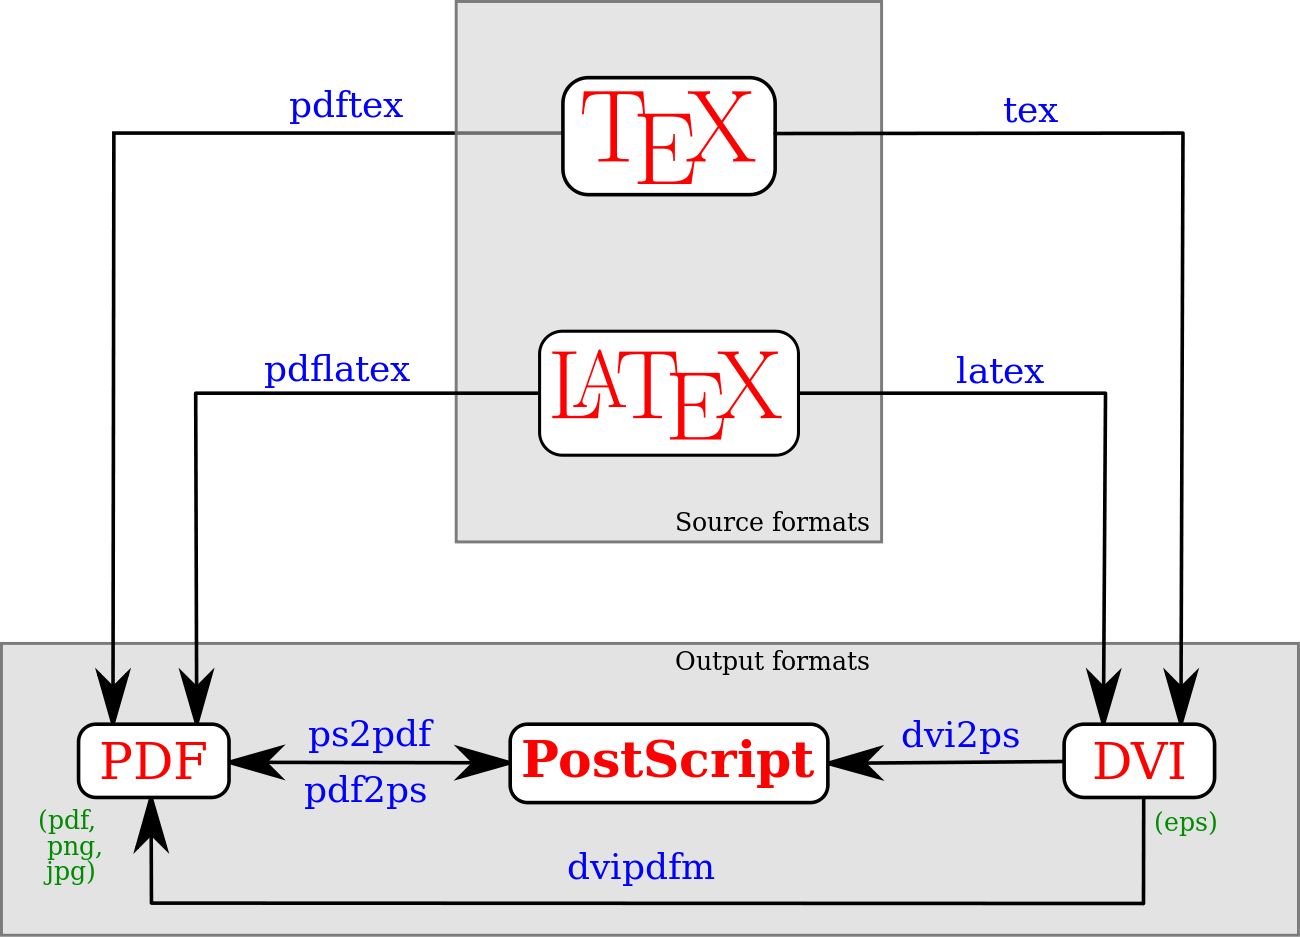
\includegraphics[width=\textheight]{latex_diagram.png}
		\end{figure}
	\end{frame}

	\begin{frame}
		\frametitle{Составные части}
		\begin{enumerate}
			\item \textbf{Файл} статьи или презентации $+$ стилевой файл.
			\item \textbf{Пакеты расширений} - дополняют функциональные возможности \LaTeX а.
			\item \textbf{Абзацы} - отделяются друг от друга пустой строкой, форматирование текста программы игнорируется.
			\item \textbf{Команды} - используются в тех случаях, когда надо изменить оформление текста,	вставить необычный символ, открыть новый раздел и т.п.
			\item \textbf{Формулы} - внутри текста и выключные.
			\item \textbf{Окружение} - указывает, что к данному фрагменту текста необходимо применить некоторый специальный тип оформления.
		\end{enumerate}
	\end{frame}
	
	\section{Программное обеспечение}
	\begin{frame}
		\frametitle{Программное обеспечение}
		Windows:
		\begin{itemize}
			\item \MiKTeX - \url{https://miktex.org/}
			\item \TeX studio - \url{https://www.texstudio.org/}
		\end{itemize}
		\par\bigskip
		Debian:
		\begin{itemize}
			\item \TeX Live - \url{https://www.tug.org/texlive/debian.html}
			\item \TeX Maker - \url{http://www.xm1math.net/texmaker/}
		\end{itemize}
	\end{frame}
	
	\section{Статья в \LaTeX}
	\begin{frame}[fragile]
		\frametitle{Простейший пример}

		\begin{lstlisting}
		\documentclass{article}
		\begin{document}
			Hello World
		\end{document}
		\end{lstlisting}
	\end{frame}

	\begin{frame}[fragile]
		\frametitle{Пример посложнее}
		
		\begin{lstlisting}
		\documentclass[12pt]{article} 
		\usepackage[utf8]{inputenc}
		\usepackage[russian]{babel} 
		\begin{document} 
			Several
			
			Examples
		\end{document}
		\end{lstlisting}
	\end{frame}	

	\section{Презентация в \LaTeX}
	\begin{frame}[fragile]
		\frametitle{Простейший пример}
		\begin{lstlisting}
		\documentclass{beamer}
		\begin{document}
		\title{Simple Beamer Class}   
		\author{Sascha Frank} 
		\date{\today} 
		
		\frame{\titlepage} 
		
		\frame{\frametitle{Table of contents}\tableofcontents} 
		
		
		\section{Section no.1} 
		\frame{\frametitle{Title} 
			Each frame should have a title.
		}
		\subsection{Subsection no.1.1  }
		\frame{ 
			Without title somethink is missing. 
		}
		\end{document}
		\end{lstlisting}
	\end{frame}

	\begin{frame}
		\frametitle{Рисунки с помощью TikZ}
		Пакет векторной графики TikZ - \url{http://www.texample.net/tikz/examples/}
		\par\bigskip
		\begin{tikzpicture}
			\draw (0,0) arc (0:270:8mm);
			\draw (0,0) arc (0:315:1.75cm and 1cm);
			\filldraw[fill=cyan, draw=blue] (0,0) -- (12mm,0mm) arc (0:30:12mm) -- (0,0);
		\end{tikzpicture}
	\end{frame}
	
	\section{Разное в \LaTeX}
	\begin{frame}
		\frametitle{Библиография}
		Библиографические системы 
		\begin{enumerate}
			\item BibTeX - старая система,
			\item Biber - новое расширение.
		\end{enumerate}
		
		
	\end{frame}
	
	\begin{frame}
		\frametitle{Онлайн редактирование}
		\begin{itemize}
			\item ShareLaTeX - \url{https://www.sharelatex.com/}
			\item LaTeXBase - \url{https://latexbase.com/}
		\end{itemize}
	\end{frame}
	\begin{frame}
		\centering
		\Huge
		Спасибо за внимание!
		\normalsize
		\par\bigskip
		\par\bigskip
		\par\bigskip
		pan@isa.ru
	\end{frame}			
\end{document}


